\chapter{Data processing}
\label{chap:processing}

\section{Epoching}
    For each trial, we considered/filtered only the spikes that occurred 500 ms before the head-entry was detected--when infrared beam of the nosepoke was interrupted--and those up to when the head was moved out of the nosepoke. 
    
    \begin{figure}
        \centering
        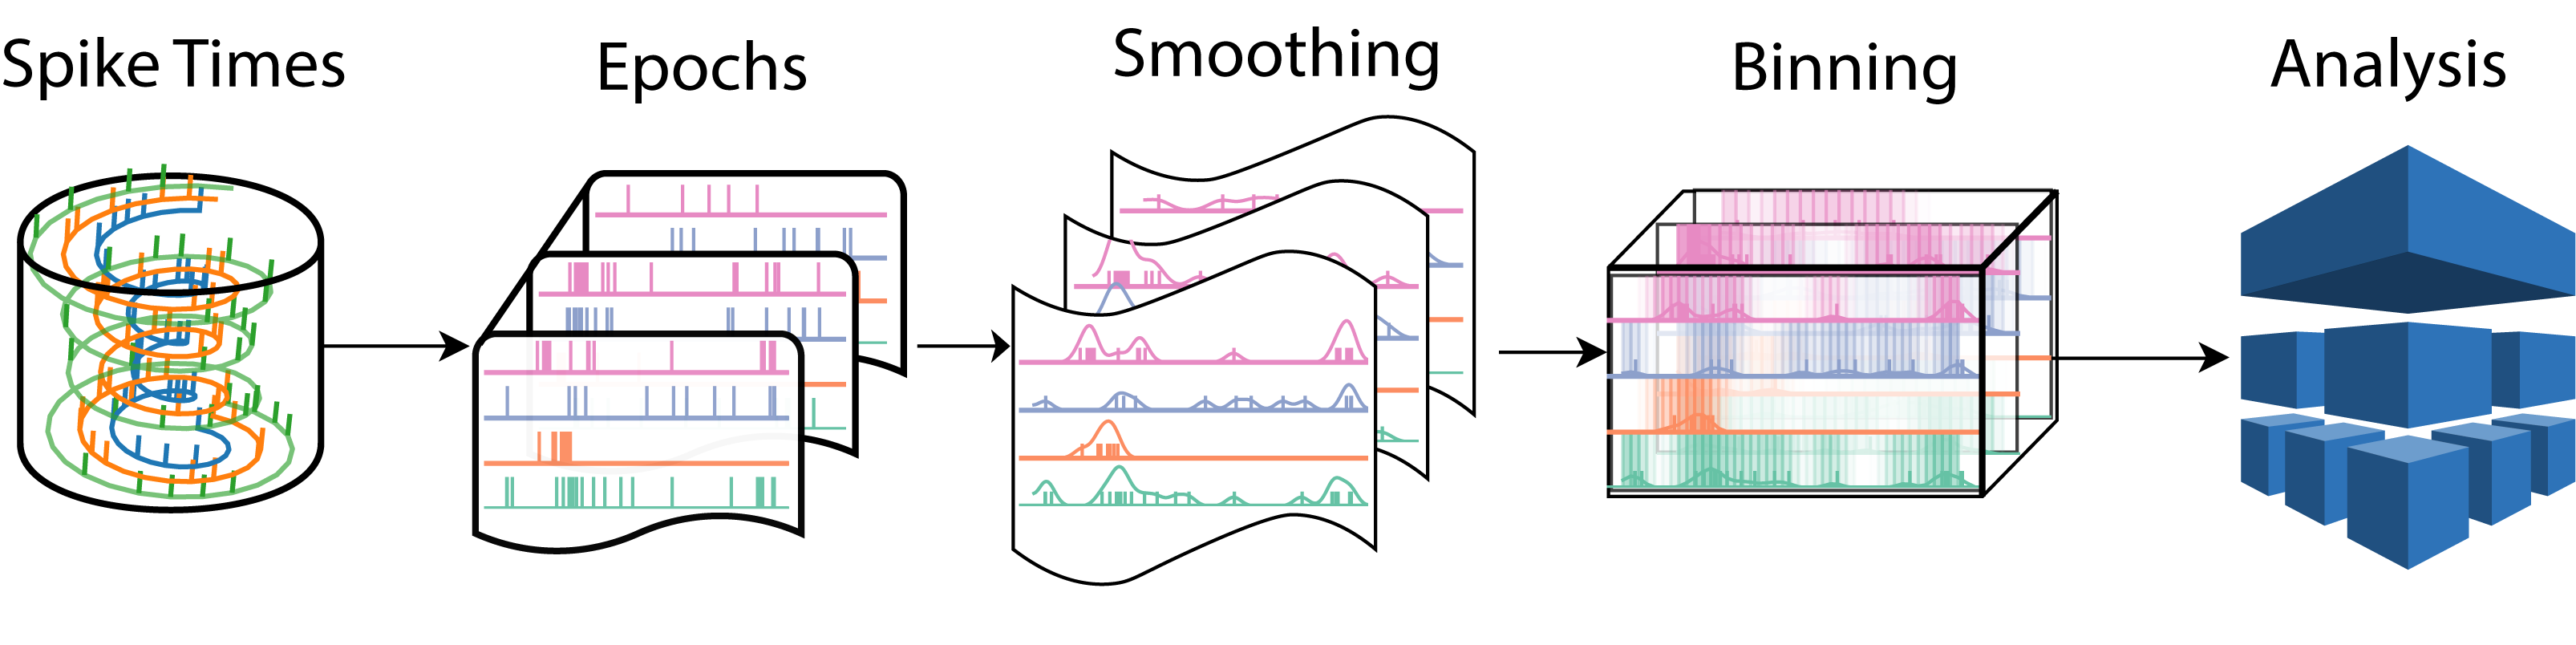
\includegraphics[width=\textwidth]{figures/Pipeline.png}
        \caption[Spike preprocessing steps]{Spike preprocessing steps: Spike times are epoched according to the nosepoke onsets, then smoothed to their estimated firing rate, and finally binned in equal-sized time bins, before being analyzed by machine learning. In the three middle steps we can see the activity of four neurons, in three different trials, through the preprocessing steps.}
        \label{fig:preproc}
    \end{figure} 
    
    % We divide spikes into their corresponding trials by using the events measured by our box. For each trial, we get all spikes that occurred between baseline (500ms before trial onset) and trial offset. This means it is possible to have the same spike in two trials, in cases when the intertrial interval is less than the baseline duration of 500ms, which was considered non-problematic.
    % \subsection{Firing rate estimation}
    % Before convolving we have to transform the time stamps into a boolean timeseries, for which we choose the precision of 1ms. Each neuron has then a time series of zeros and ones, with ones in times where the neuron was spiking.e

\section{Firing Rate estimation}
    We transformed the spike time-stamps into firing rates by convolving them with a gaussian \textit{kernel}, with standard deviation $\sigma = 100ms$ and symmetric padding, to avoid creating temporal information which would appear in the case of zero padding. After the convolution, we bin the spikes into windows of 100ms. For a given time bin we have a vector of activity, representing neurons' mean firing rate during those 100ms. Each dimension in this vector represents a different neuron.
    
    % We used three values for the standard deviation (20, 50 and 100), to assess the robustness of our analysis with respect to this parameter. To test the effects of different padding choices in estimating the firing rate, we compared the spike count (not smoothed) in 100ms bins with the firing rates measured using a gaussian kernel with standard deviation of 100ms, calculating the borders with either the default zero padding or a symmetric padding. At last we used the
    %, 50 and 20 ms. While the windows of 100 and 50 can be used for computationally expensive analysis, The window of 20ms is stored for visualization purposes.

\section{Selection}
    Engagement was assessed through the inter trial interval (ITI) of the animals. Since a single session can last more than a thousand trials, we expected that at some point the animal gets tired, in such a way that it may cease to engage in new trials immediately after the previous ones. We compared this interval between subsequent trials via visual inspection, and generously removed trials to be sure we wouldn't pollute posterior analysis with these unengaged trials.
    
    Unless otherwise specified, we selected all correct trials (t > 1.5s) for our analysis, after the removal of trials without engagement. 
    As typically done in the literature, we merged cells from all rats in most analysis, but we also performed these for each rat, to assess the consistency of our results. Each animal's first correct trial formed the first trial with increased number of (merged) cells, their second correct trial formed the second merged, and so on.

\section{Rationale}
    Here we explain why we choose symmetric padding, and assess the effects of bin size and smoothing procedure.
    
    We first assess the preprocessing steps generally used for spike time data, which consists of binning and smoothing spike times to obtain firing rates for each recorded neuron. In sum, we wanted to go from the PSTH figures (or raster plots) to the firing rates. We can see in figure \ref{fig:padding} that applying a gaussian kernel induces correlations between neighboring time points, in such a way that time points with high spike counts induce medium spike counts in neighbour time points. Without smoothing, the activity in single trials is very sparse (i.e. has few nonzero values), and since the precise spike time of a given neuron may not be so representative of its internal state, this transformation into firing rate may aid the classifier in capturing the information present in the neurons.
    
    We can also see, specially when averaging trials, how different paddings result in different estimated firing rates at the borders of the window: padding the activity with zeros biases down the average firing rate. In our posterior analysis, except when explicitly stated, smoothing was done with symmetric padding.
    
    \begin{figure}
        \centering
        \begin{tabular}{cc}
        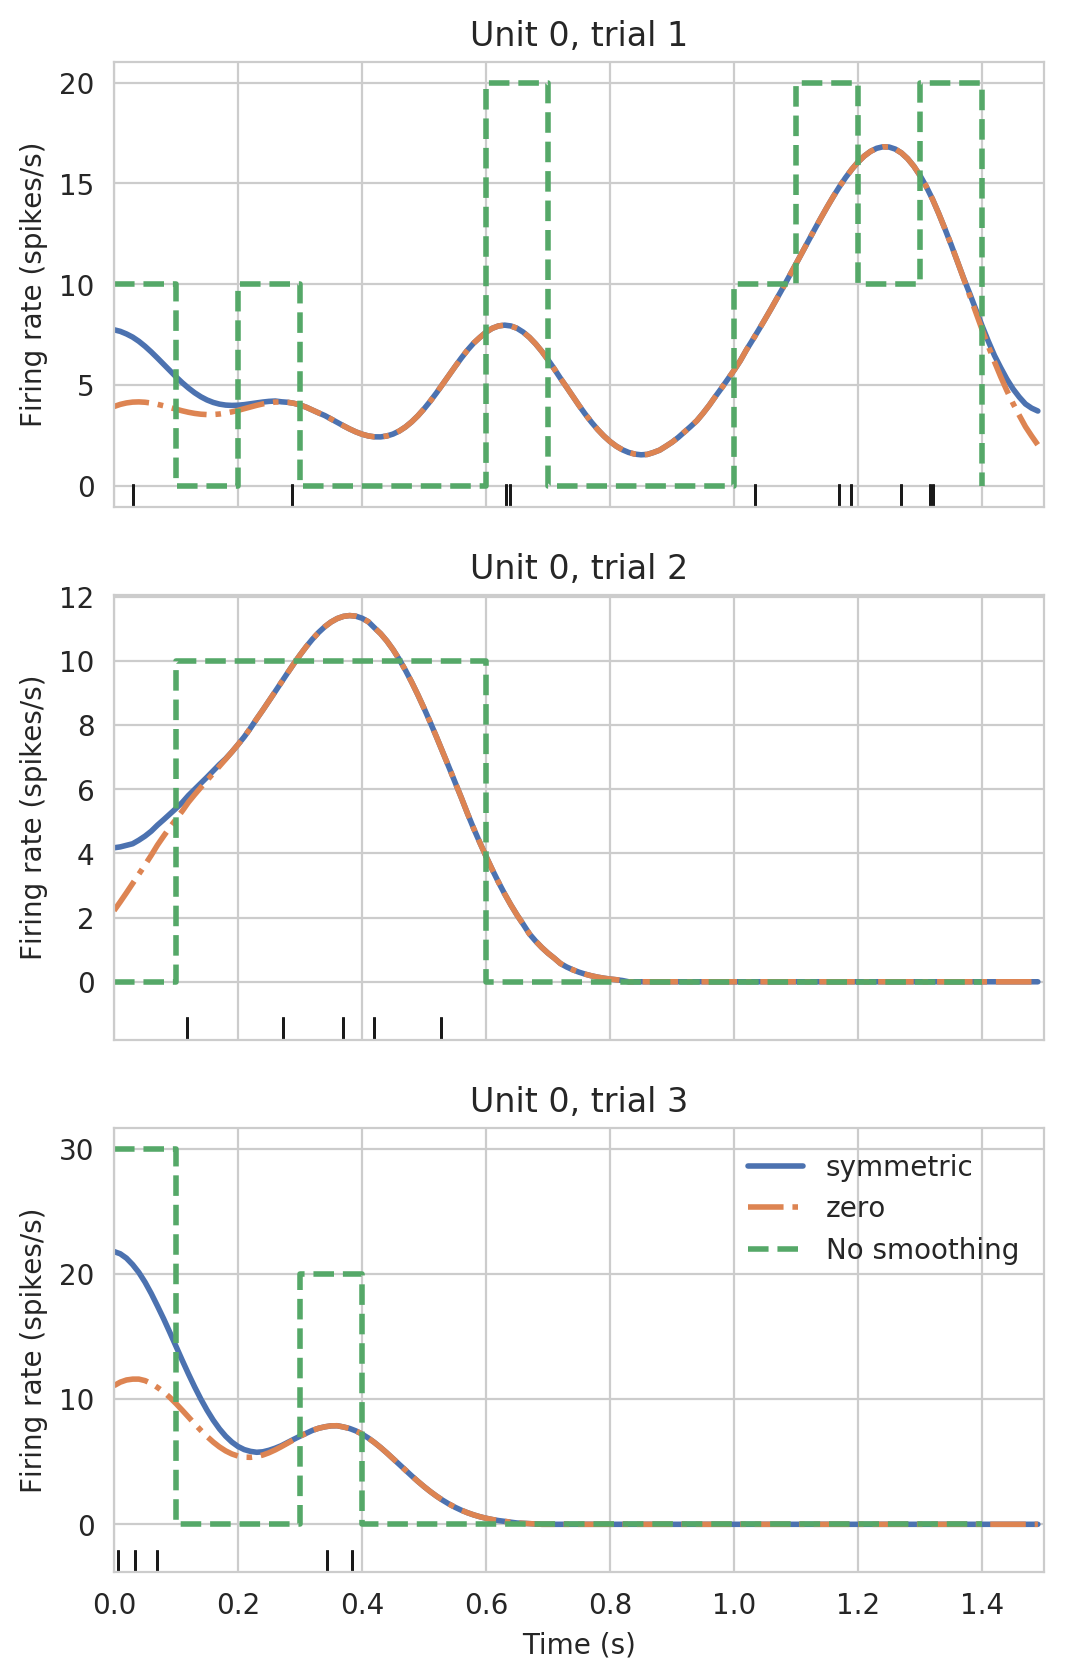
\includegraphics[width=7cm]{figures/one_with_step.png}
        & 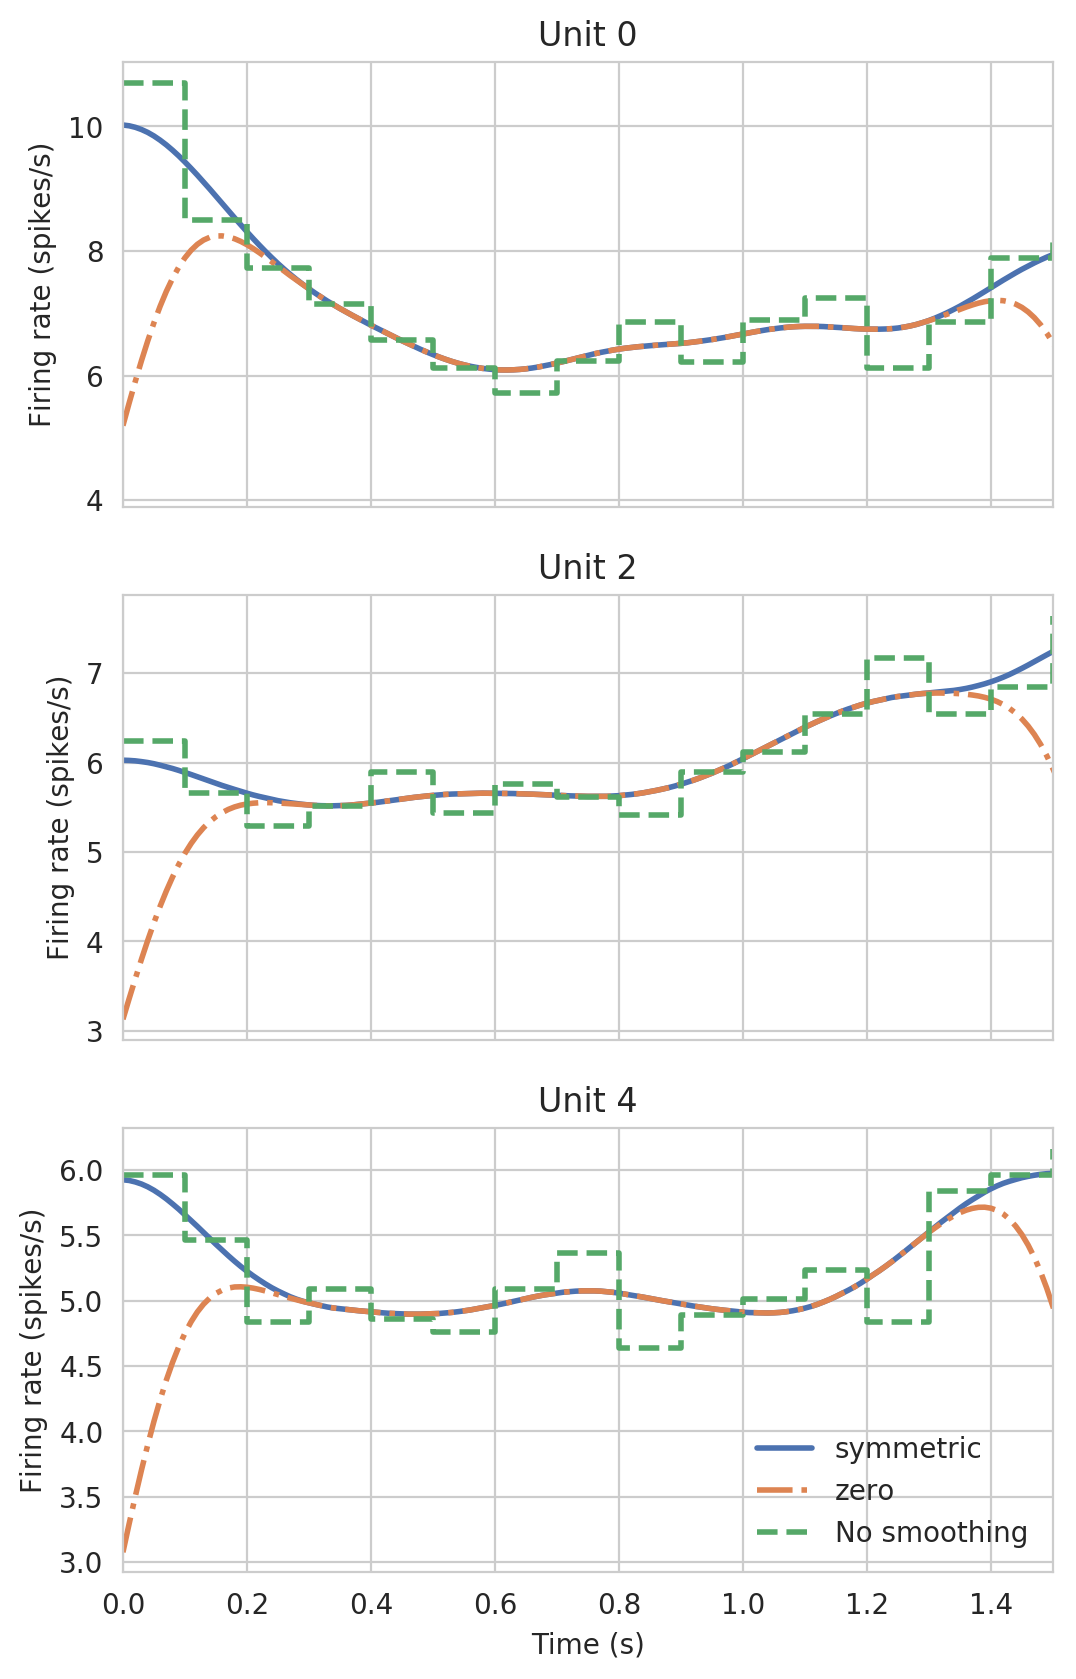
\includegraphics[width=7cm]{figures/mean_with_step.png}
        \end{tabular}
        \caption[Effect of smoothing and padding choices on the estimated firing rate.]{Effect of smoothing the spike counts with a 100ms kernel and padding choices on the estimated firing rate. Left: Single trial firing rates, Right: Mean firing rates. In the left, exact spike times appear as black ticks in the x axis.}
        \label{fig:padding}
    \end{figure} 
    
    \begin{figure}
        \centering
        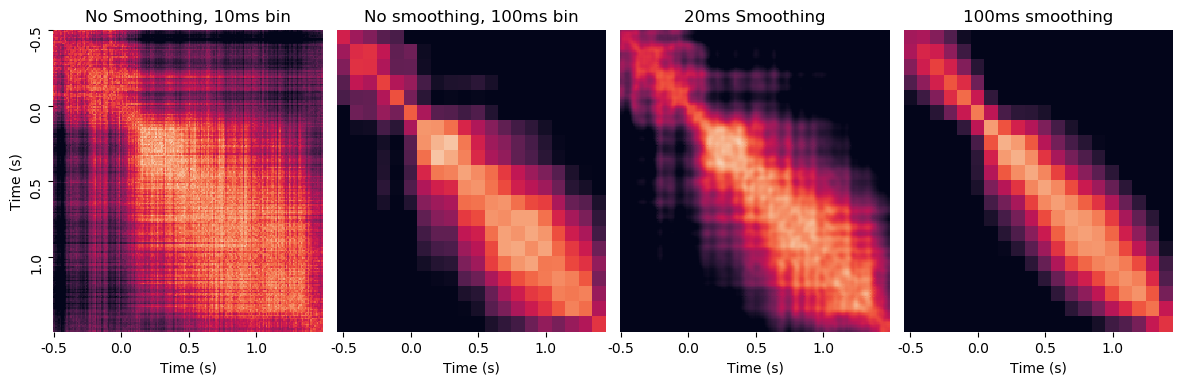
\includegraphics[width=\textwidth]{figures/similarity_comparison.png}
        \caption[Binning and smoothing assessed via similarity matrix]{Binning and smoothing assessed via similarity matrix. Spike count activity at left is binned in small and big time bins, and at the right is smoothed with a narrow and a wide gaussians.}
        \label{fig:mahalanobis_smoothing} 
    \end{figure} %No smoothing, bin10 bin100, DRRD10 and DRRD9
    
    A simple similarity analysis was used in figure \ref{fig:mahalanobis_smoothing} to measure consistency in the dynamics of neural activity. The analysis compares the activity vector of each single time point with the activity vector of another time point, measuring proximity in a space that considers less strongly dimensions in which variability is bigger. We expect to see stronger diagonals when the activity is very similar among trials, indicating that activity vectors coming from the same time point are usually near each other.
    
    In figure \ref{fig:mahalanobis_smoothing}, we can see at the left that bins that are too small can make it hard to see trial consistencies, in the case of no smoothing, because of the sparsity of spike activity. When we bin in 100ms windows, we can see that activity appears more consistent, what can be also achieved by smoothing with small kernels (e.g. 20ms). A larger kernel (100ms) makes the activity yet more consistent. 
    In all cases, it is clear that the baseline is more similar to itself, and different from the rest of the trial. This is expected since the animal is in a different state, generally approaching the nosepoke, as opposed to standing still with its nose inside. 